\section{Description}

\subsubsection*{Structure d'accueil}

J'ai donc effectué mon stage au sein du "DOT" de l'Aéroport de Bordeaux-Mérignac : Département Opérations Techniques.

Tout d'abord, la Société Aéroport de Bordeaux-Mérignac (SA ADBM) est une entreprise privée à intérêt publique.

Contrairement à ce que l'on pense, les clients de l'Aéroport ne sont pas les passagers, mais les compagnies aériennes. Ils fournissent les infrastructures aux compagnies pour un bon fonctionnement de leurs vols. Les passagers sont les clients des compagnies aériennes.\newline


\textbf{Un peu d'Histoire}\newline

L'Aéroport a été construit en 1912 après l'achat de 45 hectares par l'Etat mais l'aérogare ne connaîtra son premier visage que dans les années 1930.

\begin{figure}[hbt!]
    \begin{subfigure}{0.5\textwidth}
      \centering
      % include first image
      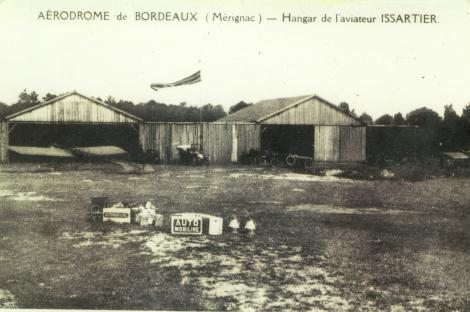
\includegraphics[width=.7\linewidth]{Images/premier.jpg}  
      \caption{Aérodrome de Bordeaux-Mérignac}
      \label{fig:aérodrome}
    \end{subfigure}
    \begin{subfigure}{0.5\textwidth}
      \centering
      % include second image
      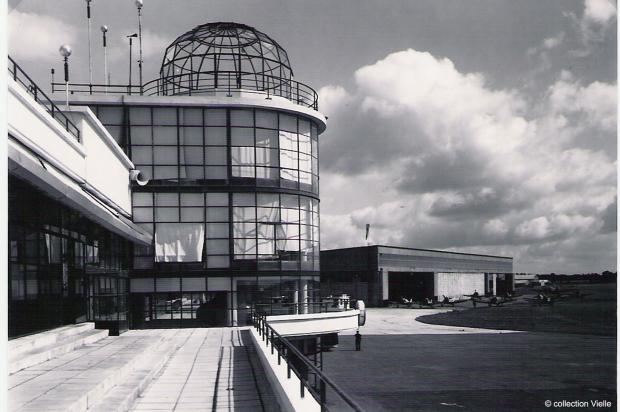
\includegraphics[width=.7\linewidth]{Images/premiere_aerogare.jpg}  
      \caption{Première Aérogare}
      \label{fig:premiereAerogare}
    \end{subfigure}
\end{figure}
De nombreux travaux se succèdent jusqu'en 2003 afin d'agrandir l'aéroport et d'y ajouter de nouveaux halls d'enregistrement et d'embarquements ainsi qu'une tour de contrôle.

En 2007, l'Etat concède l'exploitation et la gestion de l'aéroport à SA ADBM pour 30 ans. Depuis, de nombreux travaux ont été réalisés comme la création d'un nouveau parking plus économique, le hall "billi" destiné aux compagnies aériennes low-cost (Ryanair et EasyJet). Il sera par la suite agrandi en 2015.\newline

\begin{figure}[hbt!]
    \begin{subfigure}{0.5\textwidth}
      \centering
      % include first image
      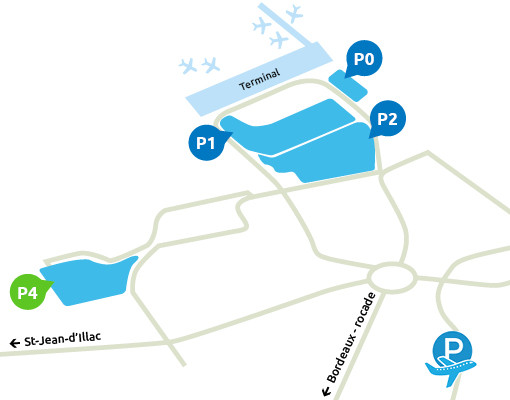
\includegraphics[width=.7\linewidth]{Images/parkings.jpg}  
      \caption{Plan des parkings}
      \label{fig:parking4}
    \end{subfigure}
    \begin{subfigure}{0.5\textwidth}
      \centering
      % include second image
      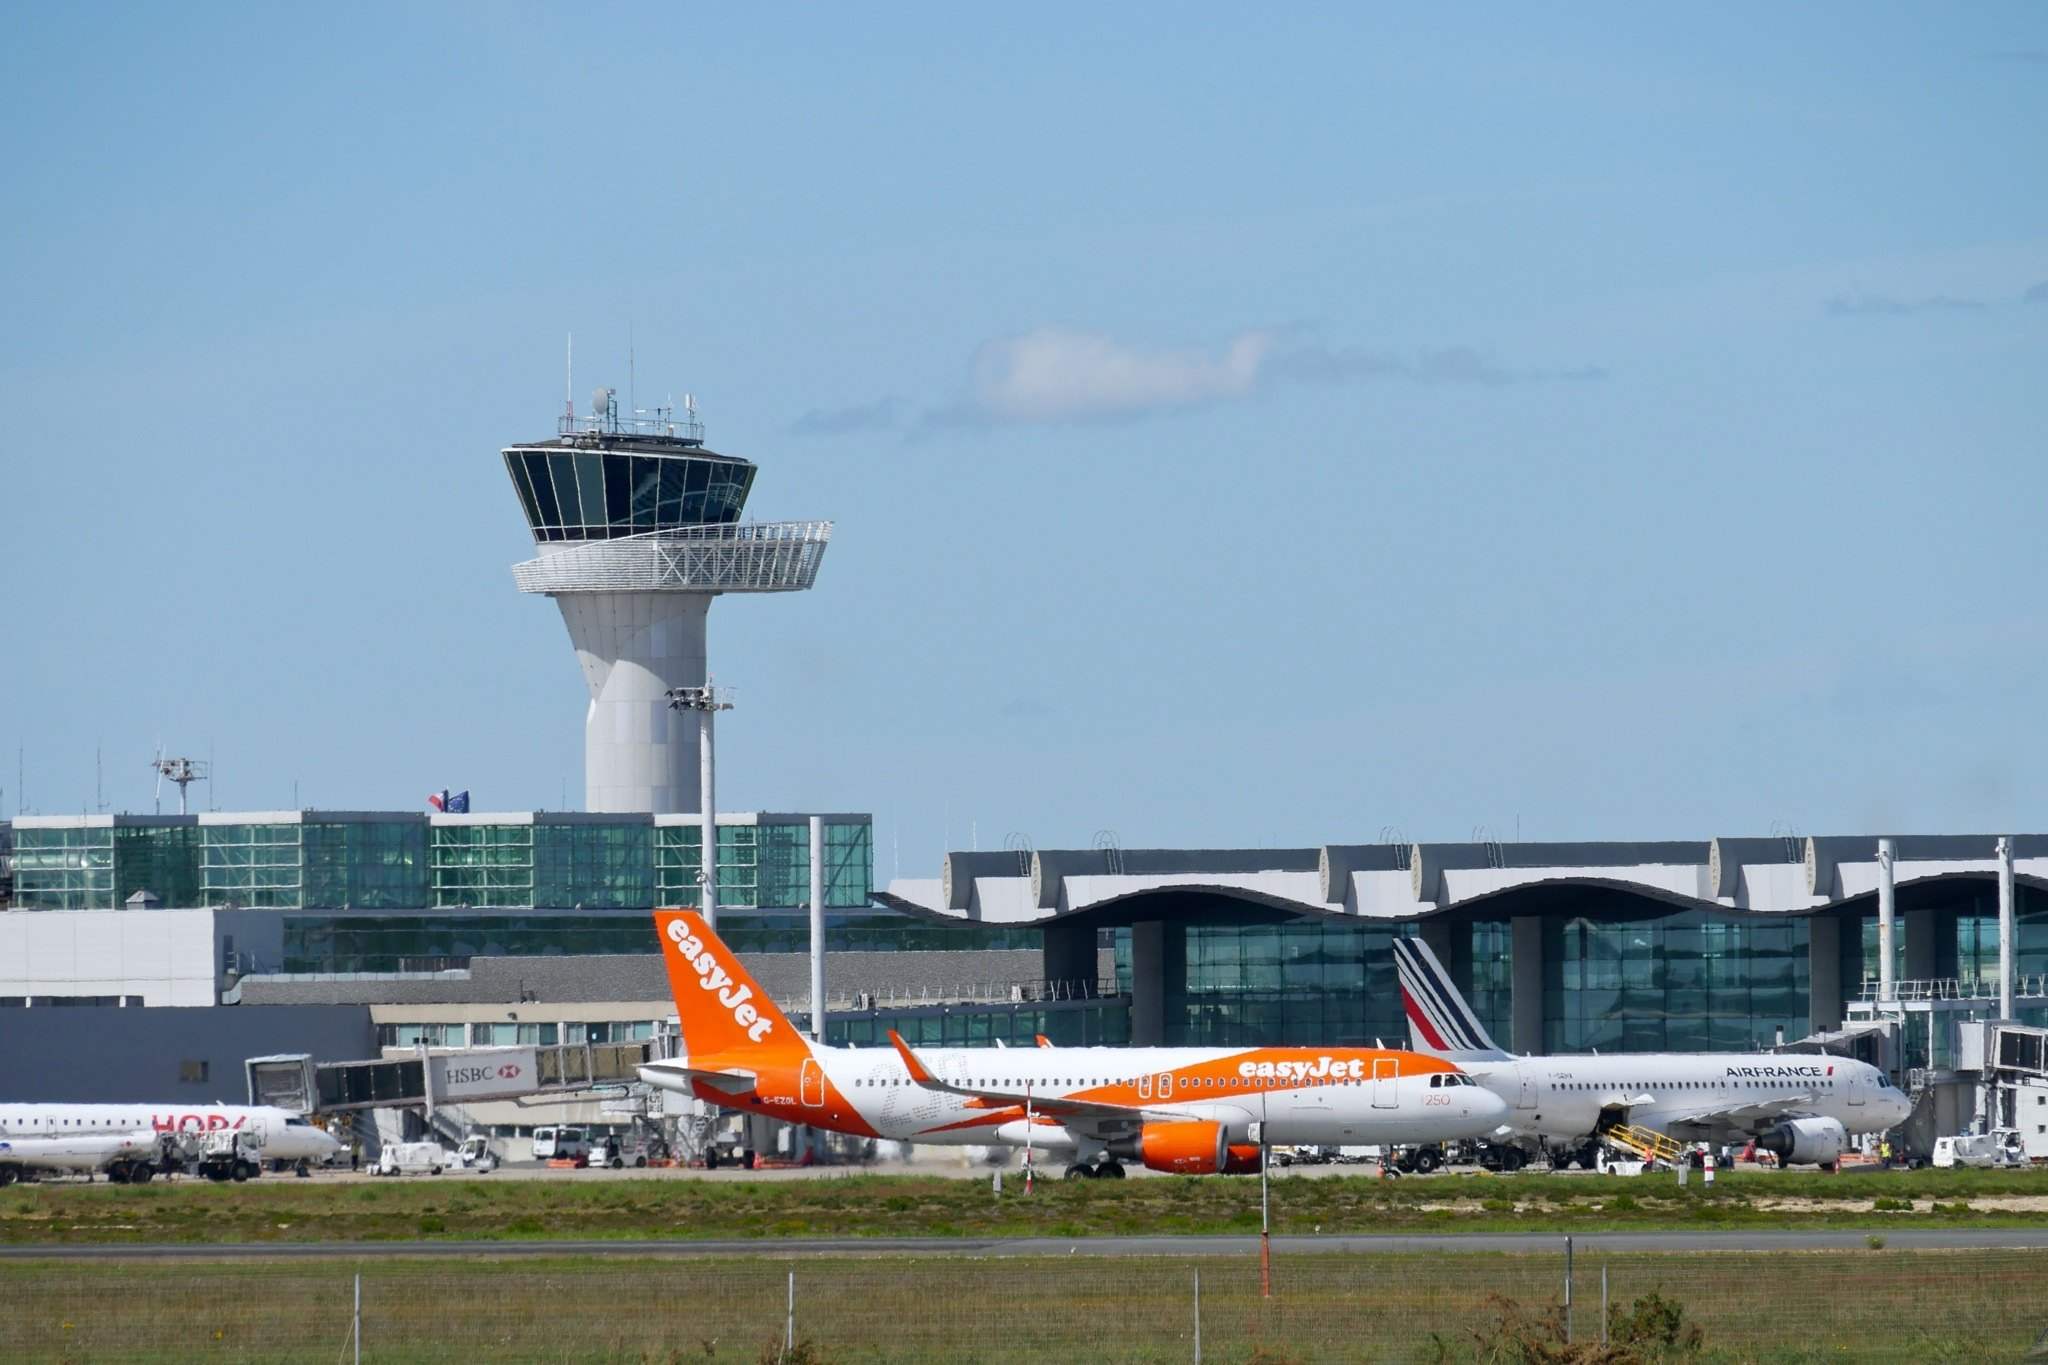
\includegraphics[width=.7\linewidth]{Images/tour.jpg}  
      \caption{Nouvelle Tour de Contrôle}
      \label{fig:tour}
    \end{subfigure}
        
    \begin{subfigure}{.5\textwidth}
      \centering
      % include third image
      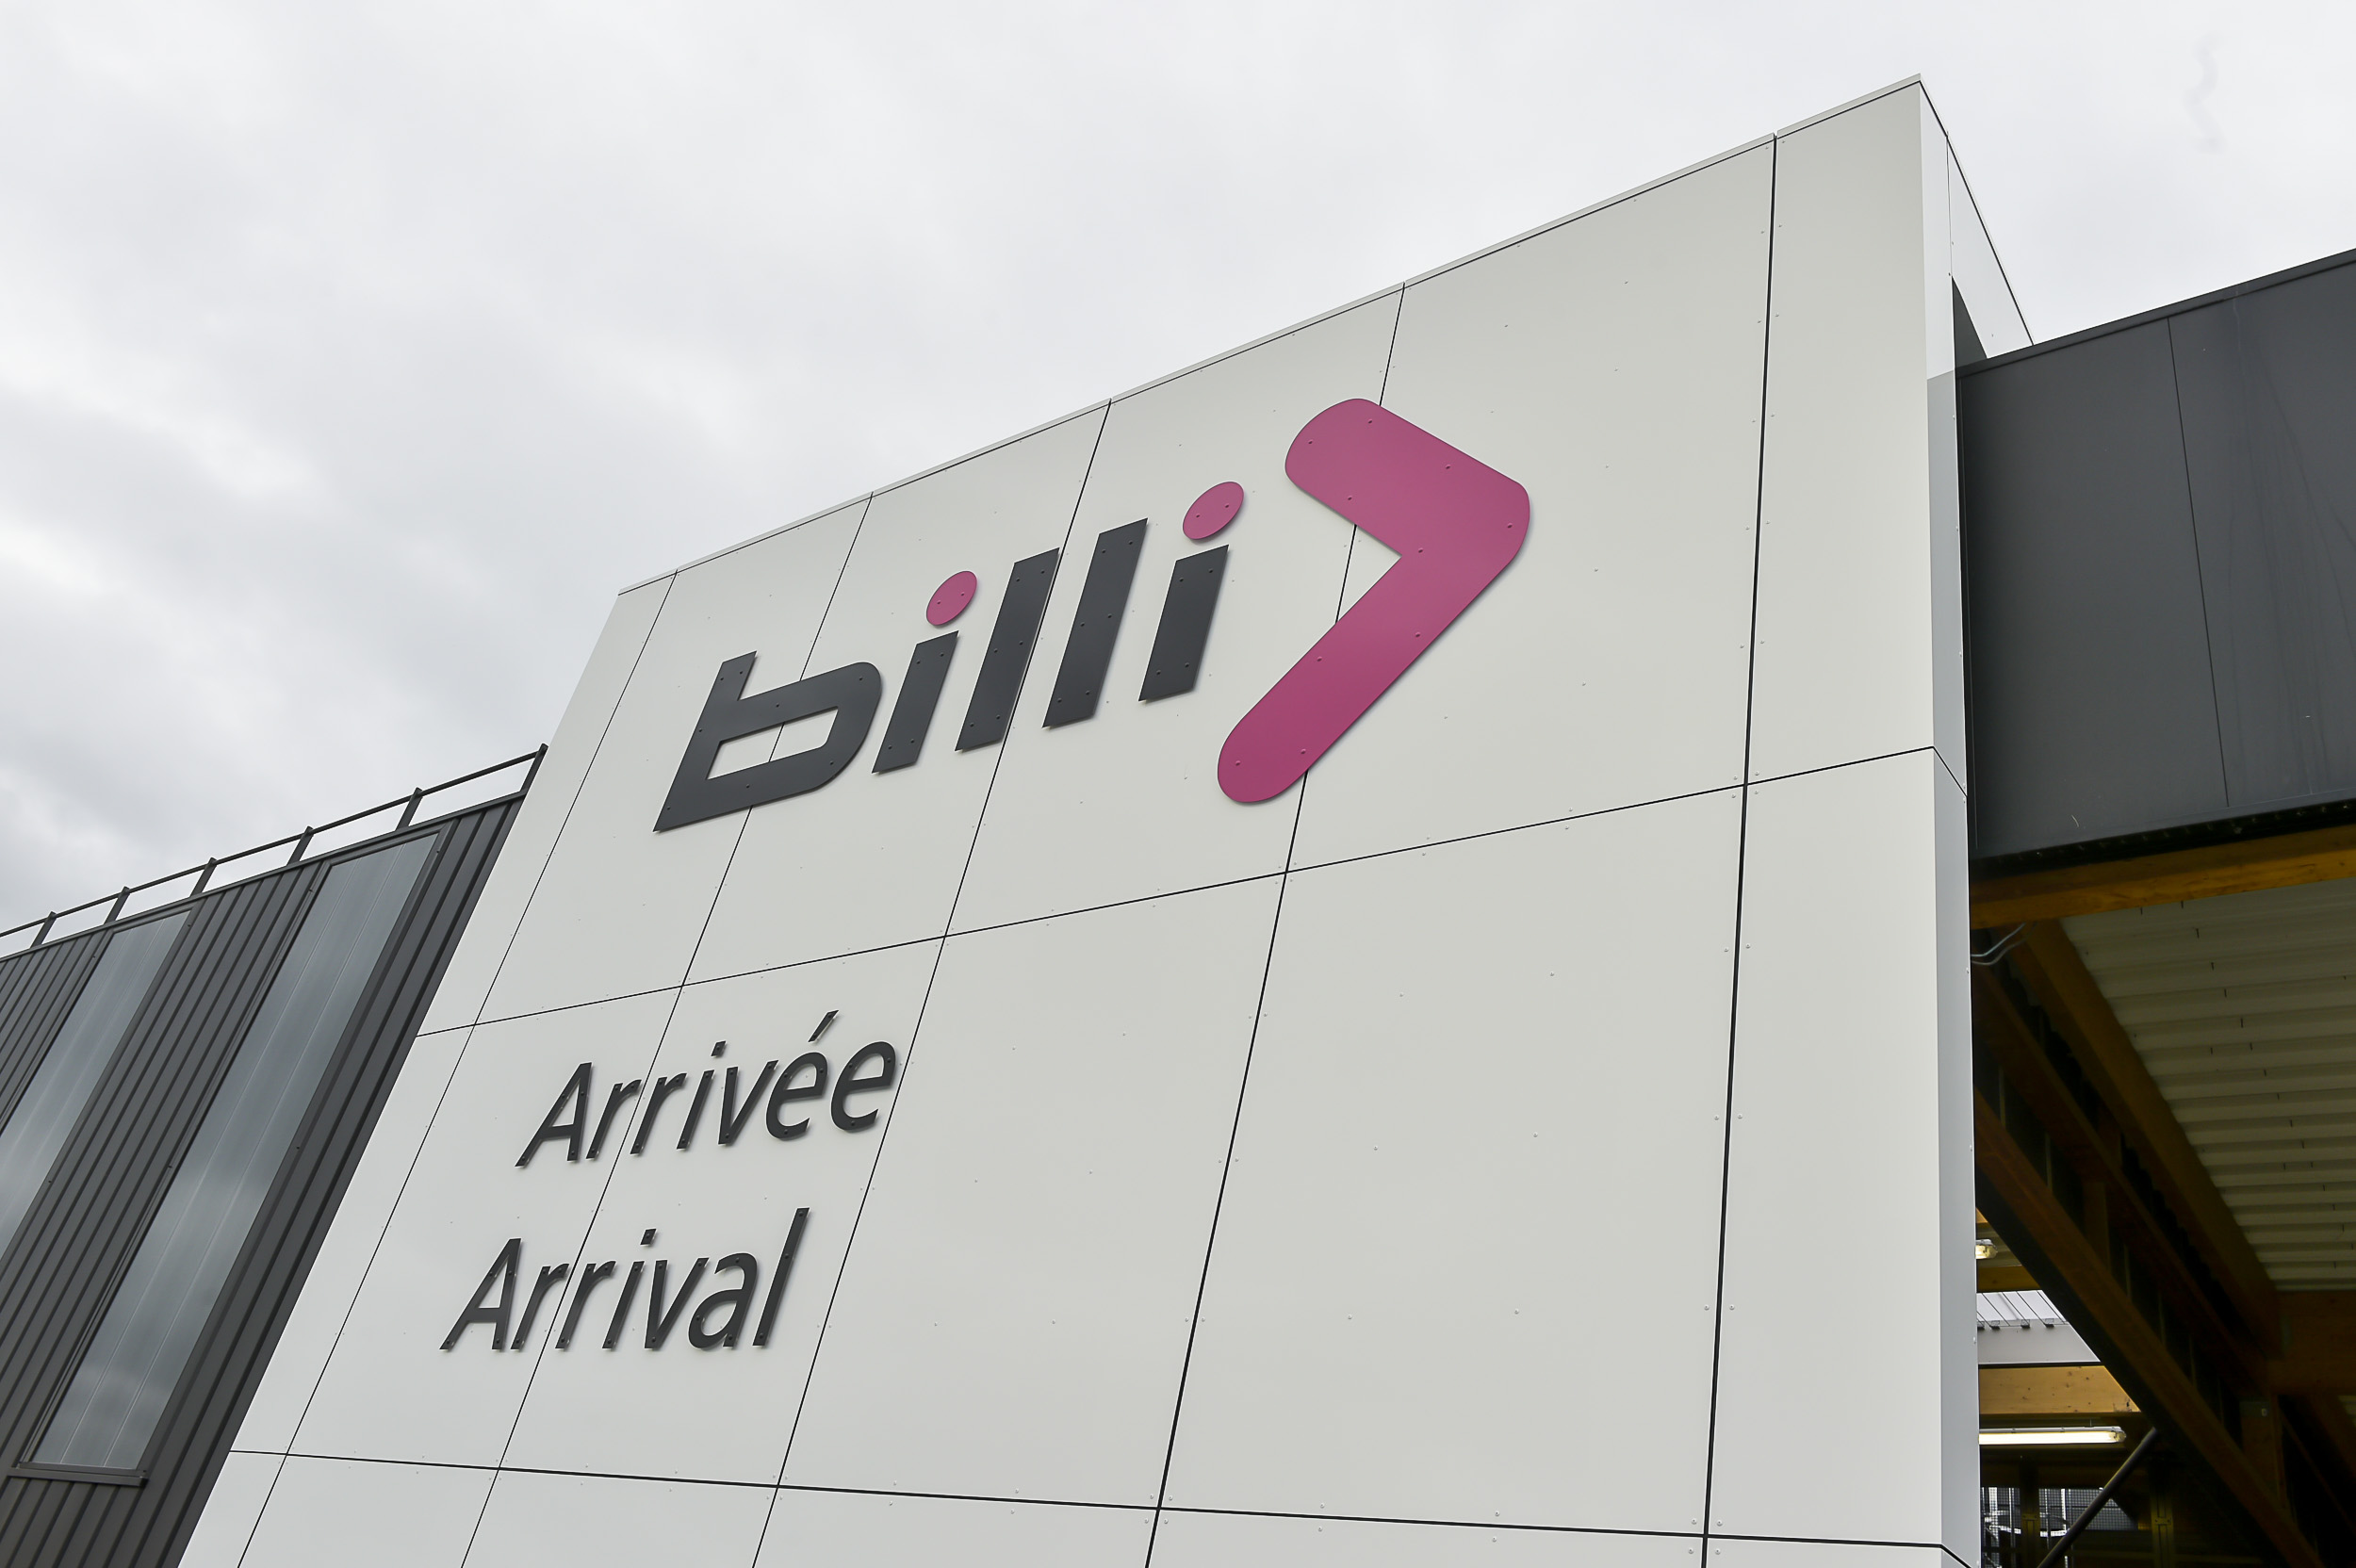
\includegraphics[width=.7\linewidth]{Images/billiext.jpg}  
      \caption{Terminal Billi}
      \label{fig:billiext}
    \end{subfigure}
    \begin{subfigure}{.5\textwidth}
      \centering
      % include fourth image
      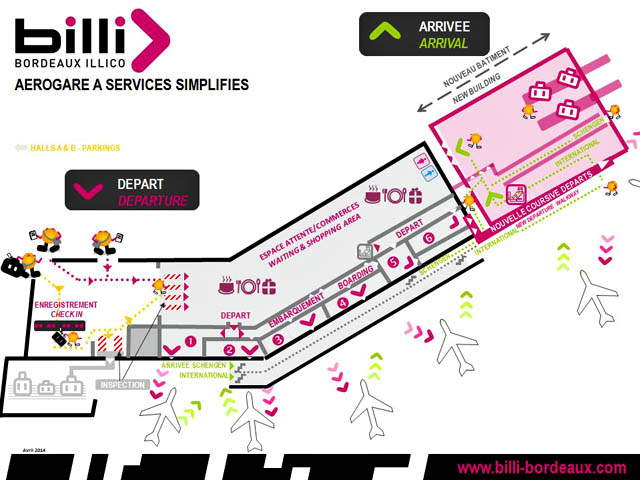
\includegraphics[width=.7\linewidth]{Images/billi.jpg}  
      \caption{Plan Billi}
      \label{fig:planBilli}
    \end{subfigure}
    \label{fig:travaux}
\end{figure}


\textbf{Infrastructures actuelles}\newline


A ce jour, la SA ADBM gère et exploite toujours l'Aéroport de Bordeaux-Mérignac.
L'aéroport possède aujourd'hui 2 pistes sécantes, 39 portes d'embarquements et 3 terminaux :

\begin{itemize}
    \item Le Hall A : National et International
    \item Le Hall B : National AirFrance uniquement
    \item Billi : National et International Low-Cost uniquement (EasyJet et Ryanair)
\end{itemize}

Les Hall A et B possèdent deux niveaux accessibles au public, le niveau 0 pour les arrivées et le niveau 1 pour les départs.

\begin{figure}[hbt!]
    \begin{subfigure}{0.5\textwidth}
      \centering
      % include first image
      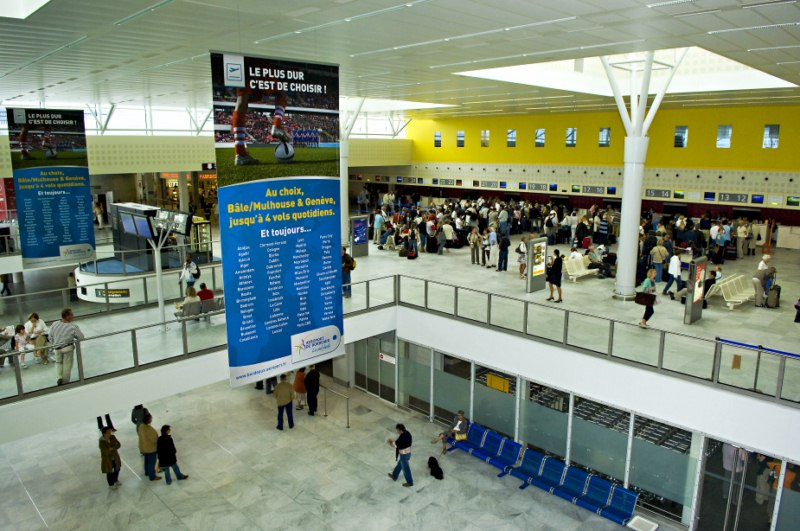
\includegraphics[width=.7\linewidth]{Images/inthalla.jpg}  
      \caption{Intérieur Hall A}
      \label{fig:inthalla}
    \end{subfigure}
    \begin{subfigure}{0.5\textwidth}
      \centering
      % include second image
      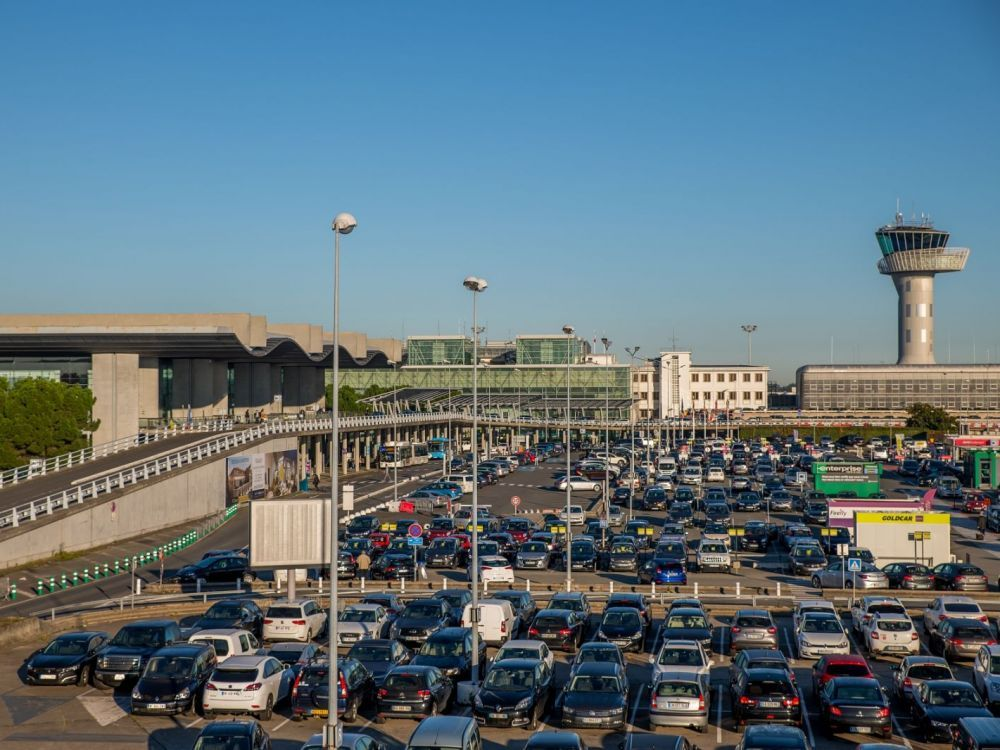
\includegraphics[width=.7\linewidth]{Images/exthalla.jpg}  
      \caption{Extérieur Hall A}
      \label{fig:exthalla}
    \end{subfigure}
        
    \begin{subfigure}{.5\textwidth}
      \centering
      % include third image
      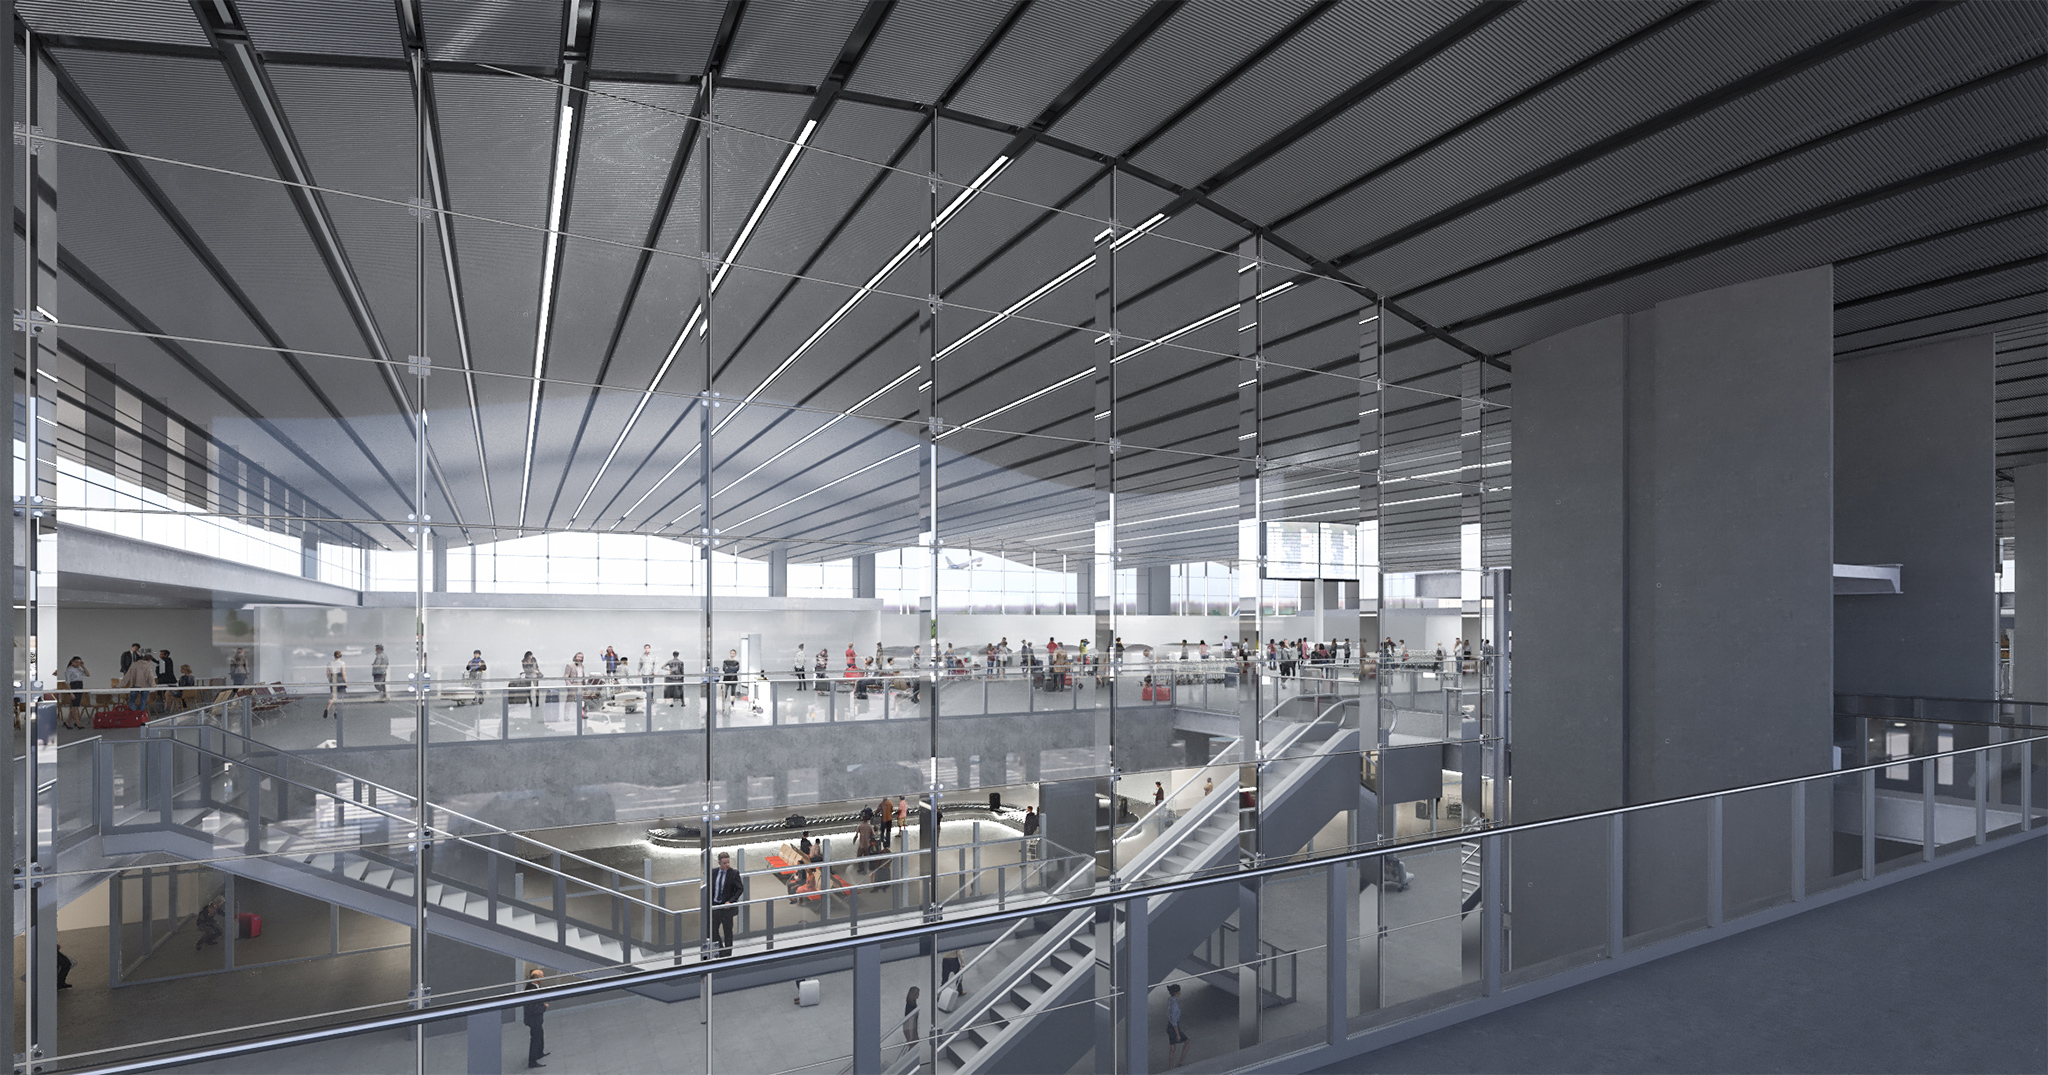
\includegraphics[width=.7\linewidth]{Images/inthallb.jpg}  
      \caption{Intérieur Hall B}
      \label{fig:inthallb}
    \end{subfigure}
    \begin{subfigure}{.5\textwidth}
      \centering
      % include fourth image
      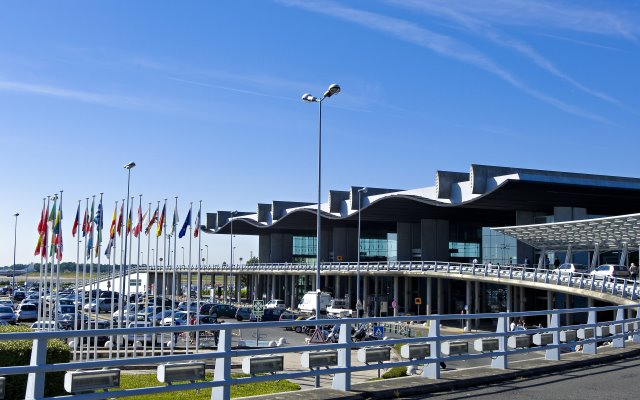
\includegraphics[width=.7\linewidth]{Images/exthallb.jpg}  
      \caption{Extérieur Hall B}
      \label{fig:exthallb}
    \end{subfigure}
    \caption{Les différents Halls}
    \label{fig:halls}
\end{figure}

\begin{figure}[hbt!]
    \centering
    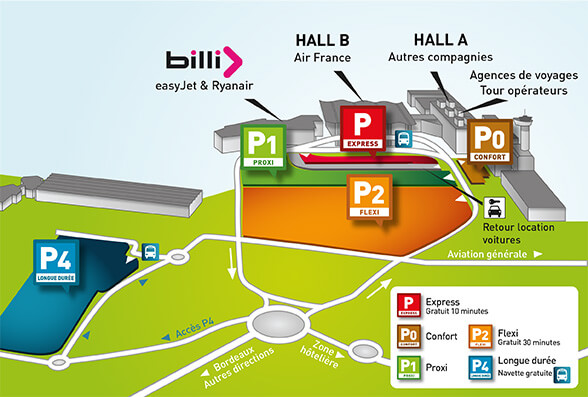
\includegraphics[width=.7\linewidth]{Images/plan.jpg}
    \caption{Plan Général}
    \label{fig:plangeneral}
\end{figure}

\newpage

\textbf{Infrastructures futures}\newline

Actuellement, deux plans d'aménagement on été engagés : Le Satellite 3 et le prolongement de la ligne A du Tramway.

Le Satellite 3 est un nouveau bâtiment construit côtés pistes du Hall A afin d'augmenter le nombre de portes d'embarquements pour l'international.

La livraison de ce bâtiment est prévue pour fin août 2021.\newline

\begin{figure}[hbt!]
    \centering
    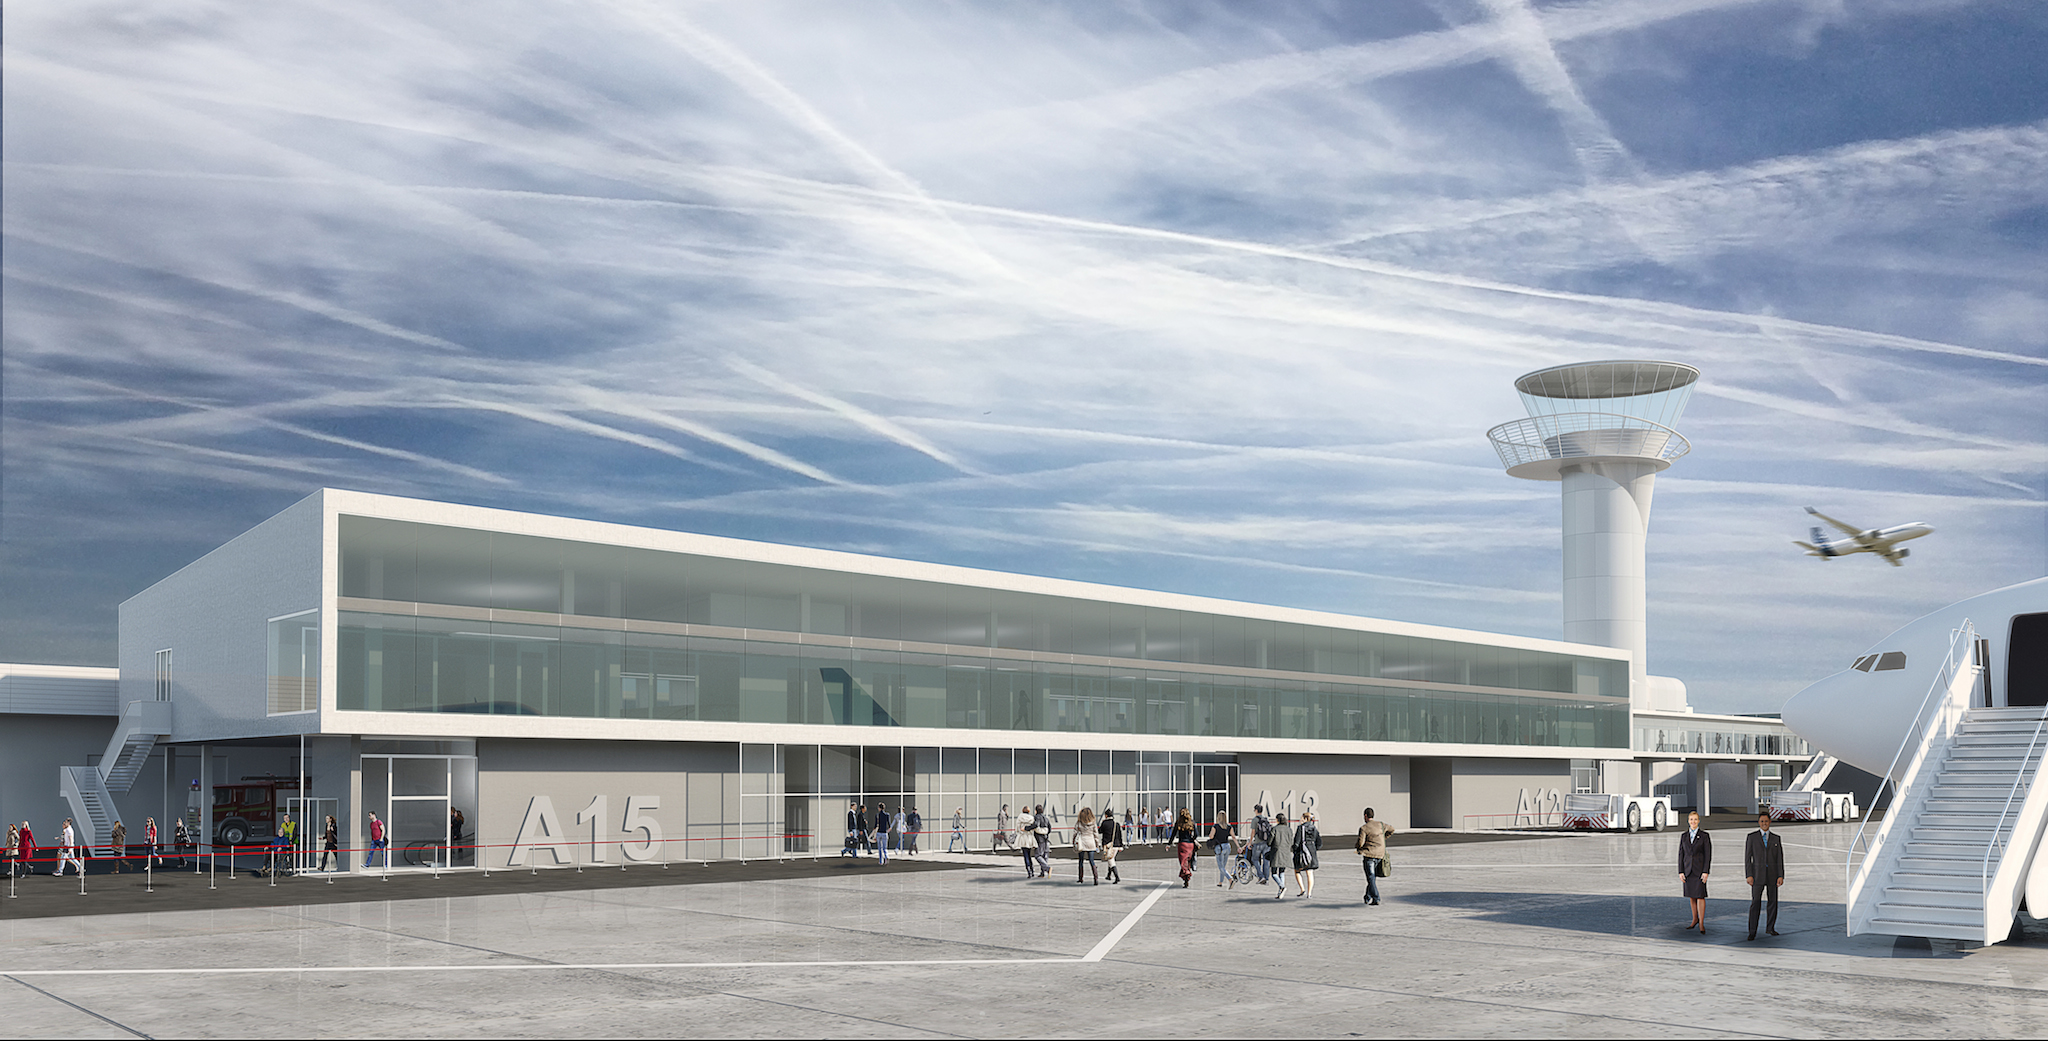
\includegraphics[width=12cm]{Images/satellite3.jpg}
    \caption{Futur Satellite 3}
    \label{fig:sat3}
\end{figure}

En partenariat avec Bordeaux Métropole, SA ADBM a engagé des travaux qui visent à rendre l'accès à l'aéroport plus simple. La ligne de tram A est donc prolongée de 6 stations avec le Terminus au pied des aéroports. Ces travaux ont été lancés en 2019 et la livraison est prévue pour automne 2022.\newline

\begin{figure}[hbt!]
    \centering
    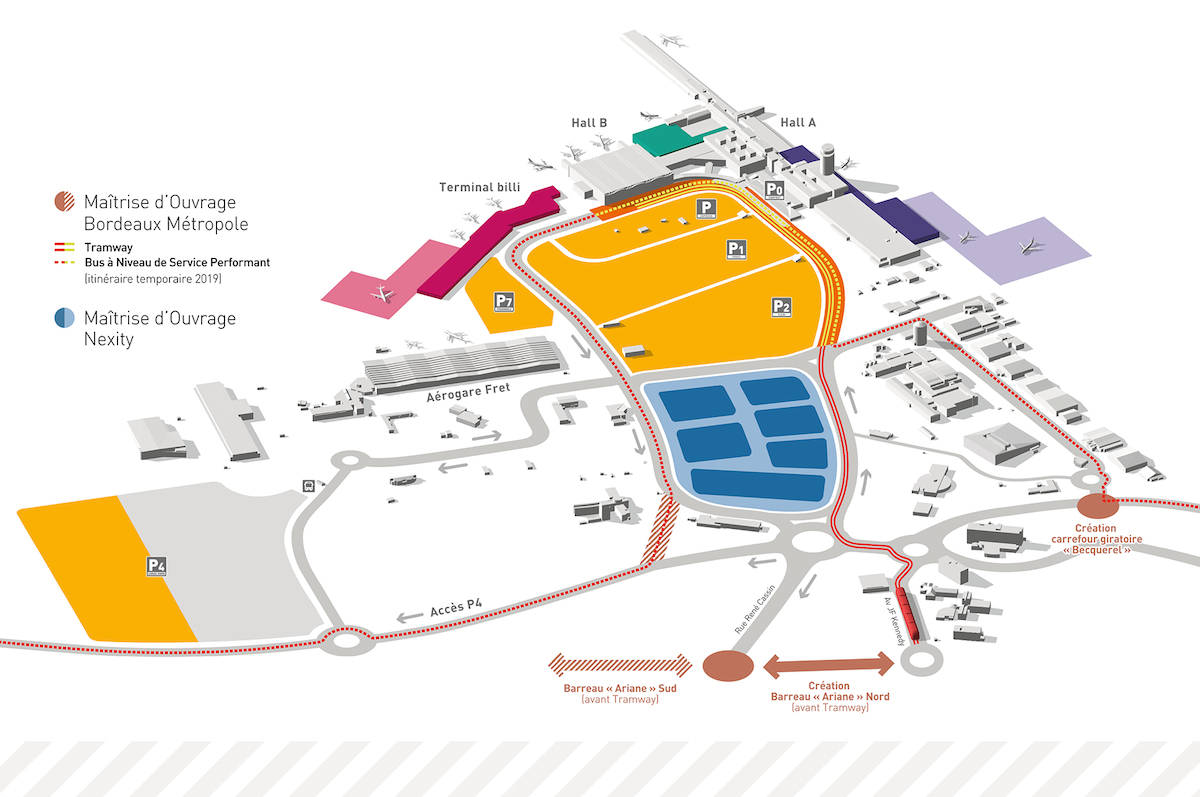
\includegraphics[width=14cm]{Images/tramway.jpg}
    \caption{Plan Futur Tram}
    \label{fig:futurtram}
\end{figure}

\newpage

\textbf{Chiffres clés}\newline

L'aéroport de Bordeaux-Mérignac a fait voyager près de 7,7 millions de passagers en 2019. Cela correspond à une croissance +134\% par rapport à 2018 :

\begin{figure}[hbt!]
    \centering
    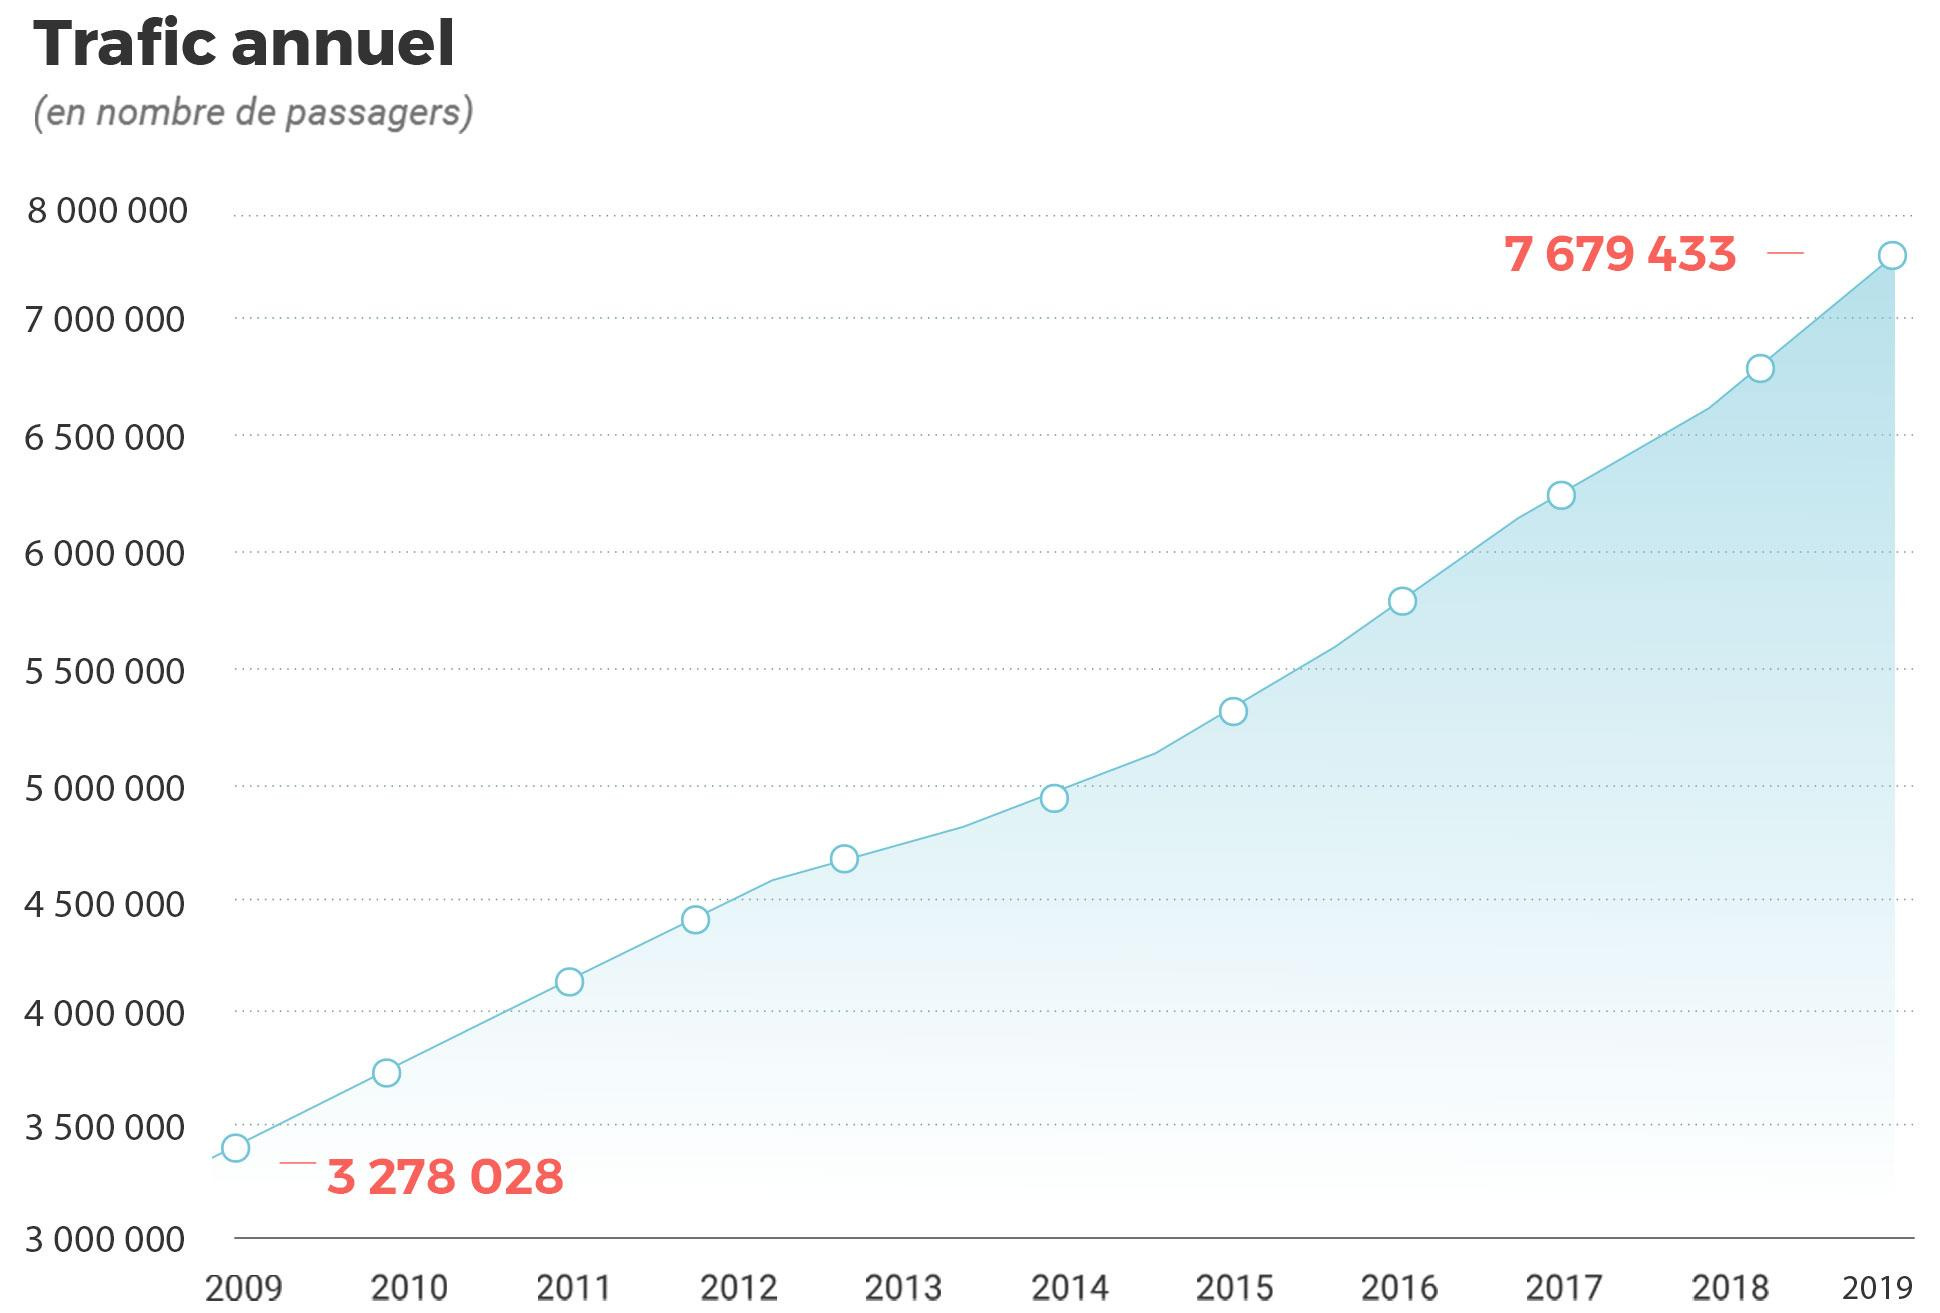
\includegraphics[width=12cm]{Images/trafic.jpg}
    \label{fig:trafic}
\end{figure}

Avant la pandémie de COVID-19, l'aéroport avait pour but de faire voyager 10 millions de passagers en 2023.

En 2019, 34 compagnies aériennes ont opéré des vols, avec un total de 163 lignes directes reliées à 31 pays différents.
De plus, plus de 125 000 tonnes de fret ont été acheminées grâce aux cargos.

C'est également un bassin d'emploi important puisque plus de 8000 personnes travaillent sur la plateforme aéroportuaire (dont 200 SA ADBM).
94 établissements sont présents sur site : entreprises, commerces, industries et organismes publics.

\subsubsection*{Personnes impliquées}


Mon tuteur était Serge CLARY, Chef de Projet Informatique, et ma supérieure Nathalie CORDEAU, Chef du Service Organisation, Informatique, Systèmes Industriels au sein du département.\footnote{Tous les organigrammes disponibles en Annexe}

J'ai travaillé en proche collaboration avec :\newline

\begin{itemize}
    \item Monsieur Marc RIVAULT : Administrateur Systèmes, Réseaux et Bases de données,
    \item Monsieur Gurvan QUENET : Responsable Sécurité des Systèmes d'Information,
    \item Monsieur Kamal MAHAMOUD : Technicien Support Informatique,
    \item Monsieur Yannick VALERY : Administrateur Systèmes, Réseaux et Bases de données.
\end{itemize}

J'ai également été reçue par :

\begin{itemize}
    \item Monsieur CABANNE Olivier : Attaché Relations Riverains et Environnement,
    \item Madame COLAS Fabienne : Coordinateur Piste.
\end{itemize}


L'avantage d'une entreprise avec une grande variété de postes, est que j'ai pu constater à quel point l'informatique est essentiel dans tous les services, autant sur l'aspect logiciel que matériel.

\subsubsection*{Activités}

Les salariés de l'aéroport étant toujours sur Office 2010, ma première mission a été d'analyser les différences entre Office 2010 et 2019 afin de savoir quel type de formation ou documentation pourrait accompagner la transition, et ensuite de la réaliser.
J'ai donc créé un document détaillé de tous les changements entre ces versions, puis ensuite un "flyer" les résumant de manière simplifiée.\newline

Ma seconde mission était de mettre à jour des ordinateurs "CREWS", les passer de Windows 7 à Windows 10 en réinstallant d'autres logiciels. En banque d'enregistrement, ce sont des ordinateurs qui permettent d'enregistrer les bagages en soute et d'imprimer leurs identifications à partir d'un scan de la carte d'embarquement du passager.
J'ai commencé à faire quelques manipulations sur les ordinateurs CREWS : Mise à jour du BIOS, Installation de Windows à partir d'un logiciel de gestion : Ivanti.
Cependant je n'ai jamais pu les installer, des problèmes techniques ont été repérés plus tard dans l'installation, et nous avons donc dû suspendre le projet.\newline

Durant le premier confinement, certains salariés se sont vus attribués un ordinateur portable afin de faire du télétravail. Or plusieurs vols ont été enregistrés chez ces personnes, et au délà de la perte financière, la perte du disque dur représentait une perte d'informations internes et donc un problème de sécurité.
Il fallait donc régler le problème afin de ne pas risquer une fuite de données, CRYHOD était la solution. CRYHOD est un logiciel de cryptage de données de disques durs.
Gurvan QUENET, le Responsable Cybersécurité de l'aéroport m'a donc donné la mission d'installer ce logiciel sur les ordinateurs portables des salariés afin de sécuriser les disques durs et protéger les données de l'aéroport.
J'ai pu l'effectuer sur quelques postes, mais Monsieur QUENET m'a demandé d'arrêter à cause d'un problème de compatibilité sur certains logiciels, la mise en place a donc été retardée.\newline

Enfin, après l'annonce du confinement national en mars 2020, des outils informatiques ont été prêtés : Postes, Ecrans, Périphériques.
Ma dernière mission était de passer dans tous les bureaux de l'aéroport et de recenser le matériel présent avant de comparer avec celui prêté dans la base de données afin de vérifier que tout le monde a bien ramené les outils prêtés.

\newpage

\subsubsection*{Démarche Responsabilité Sociale de l’Entreprise}


Lorsque l'on pense à un aéroport ou même au milieu aéronautique en général, on ne pense pas à une bonne gestion de l'environnement.
Et pourtant, comme toute entreprise, l'Aéroport de Bordeaux-Mérignac pratique une politique RSE.

J'ai pu rencontrer un des responsables du Service Environnement et Relations Riverains : Monsieur Olivier CABANNE.

En effet, l'entreprise se rend compte que ses activités sont des nuisances pour les riverains et l'environnement. 

Des points mensuels sont envoyés aux riverains, avec les résultats des différentes actions menées et des statistiques sur la trafic.

La Commission Consultative de l’Environnement (CCE) est l’instance de référence consultée sur toute question d’importance relative à l’aménagement ou à l’exploitation de l’Aéroport de Bordeaux pouvant avoir une incidence sur l’environnement. Ces réunions réunissent : 

\begin{itemize}
  \item Le Service Environnements et Relations Territoriales de l'Aéroport de Bordeaux-Mérignac,
  \item Les Élus Locaux,
  \item Les Associations de Riverains.
\end{itemize}

Suite à ces réunions, SA ADBM propose de nombreuses solutions.\newline

\textbf{Riverains}\newline

Concernant les riverains, l'aéroport a conscience que de vivre proche d'un aéroport apporte beaucoup de points négatifs.
Plusieurs actions ont été menées afin de réduire au maximum la gêne occasionée par les activités aériennes, comme Aérovision.

\begin{figure}[hbt!]
  \centering
  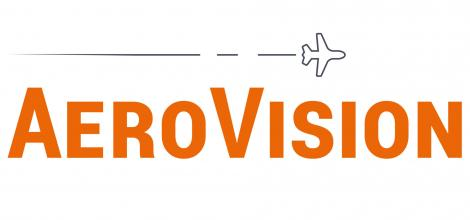
\includegraphics[width=5cm]{Images/logo_aerovision.jpg}
  \label{fig:logoaerovision}
\end{figure}

La plus grande plainte des riverains est le bruit occasioné par les avions qui volent à basse altitude afin d'atterir ou de décoller.
Le bruit des aéronefs sont soumis à une loi, le bruit capté au sol ne doit pas dépasser les 70 dB. Plusieurs associations de riverains se plaignaient que certains avions dépassaient cette réglementation.\newline

Le service informatique a donc créé AEROVISION. Ils ont été poser des stations de mesure de bruit dans des endroits habités dans la continuité des pistes.

Cet outil accessible en ligne est une carte de l'aéroport et de ses environs avec la représentation des stations ainsi que leur décibel mesuré lorsqu'un avion passe au dessus. Les trajectoires vertes sont les arrivées, et bleues les décollages.

\begin{figure}[hbt!]
  \centering
  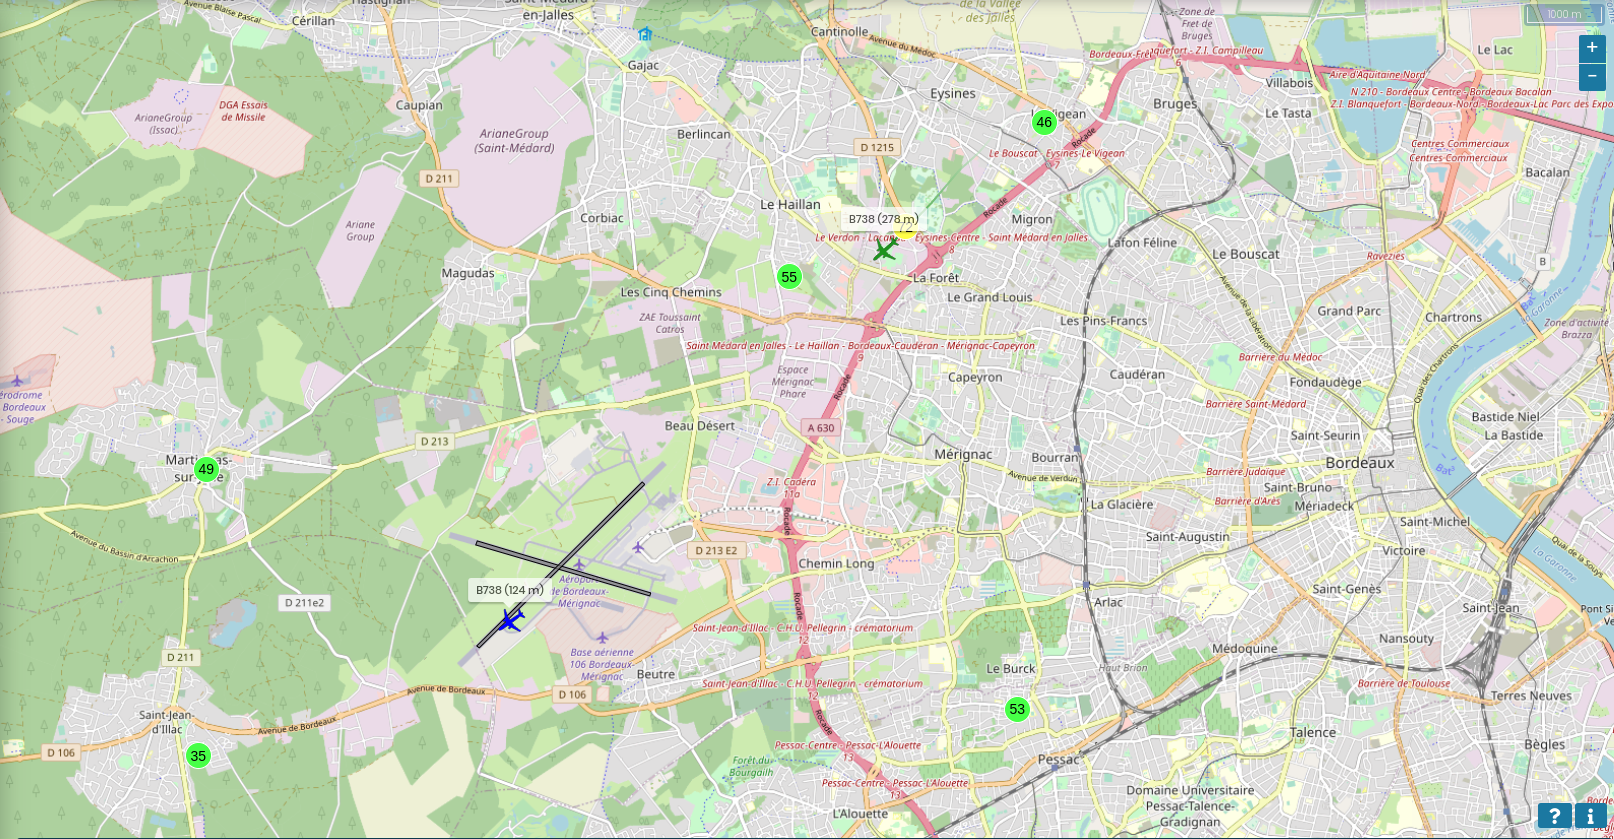
\includegraphics[width=17cm]{Images/aerovision.png}\newline
  \caption{Interface}
  \label{fig:interfaceaerovision}
\end{figure}

Un mode "Historique" est également disponible, grâce à une sélection de 30 minutes, l'utilisateur peut vérifier les informations sur des vols antérieurs.

Pour des raisons de sécurité, AEROVISION a 30 minutes de décalage avec la réalité et n'affiche que les vols civils.

Le projet AEROVISION est disponible à l'adresse : https://trajectoires.bordeaux.aeroport.fr/appmap\newline

De plus, en cliquant sur un avion sur la carte on peut obtenir des informations sur celui-ci : Modèle, Compagnie, Trajectoire, Informations d'approche et bruit total.
Une autre fonctionnalité a été créé pour les riverains : "Mon Habitation". Cette fonctionnalité permet de placer sa maison sur la carte grâce à la géolocalisation ou simplement en cliquant sur la carte.

\begin{figure}[hbt!]
  \begin{subfigure}{0.5\textwidth}
    \centering
    % include first image
    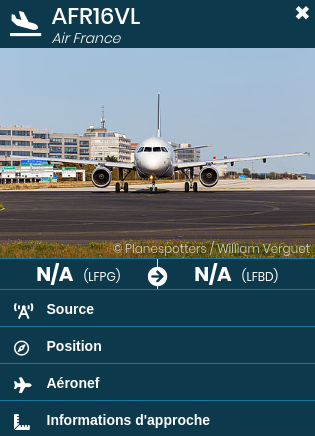
\includegraphics[width=.7\linewidth]{Images/aerovisioninfo.png}  
    \caption{Menu Informations Aéronefs}
    \label{fig:aerovisioninfo}
  \end{subfigure}
  \begin{subfigure}{0.5\textwidth}
    \centering
    % include second image
    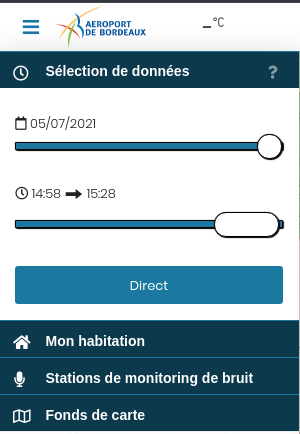
\includegraphics[width=.7\linewidth]{Images/aerovisionmaison.png}  
    \caption{Menu "Mon Habitation"}
    \label{fig:aerovisionmaison}
  \end{subfigure}
\end{figure}

Concernant les riverains et le bruit, une autre action a été menée : L'Aide à l'Insonorisation.
C'est une aide financière destinée aux habitants des quatres communes touchées par ce problème : Mérignac, Le Haillan, Eysines et Saint-Jean-d'Illac. Elle prend en charge complètement les travaux de rénovation pour insonoriser l'hôtel ou le logement.

Pour bénéficier de cette aide financière, il faut être situé dans une des zones du Plan de Gêne Sonore en vigueur, et avoir un permis de construire datant d'avant la création du Plan d'Exposition au Bruit.\footnote{Les deux plans sont disponibles plus grands en annexe}
Le but étant de dédommager les personnes s'étant installées près de l'aéroport avant de vraiment connaître la gêne sonore.

\begin{figure}[hbt!]
  \begin{subfigure}{0.45\textwidth}
    \centering
    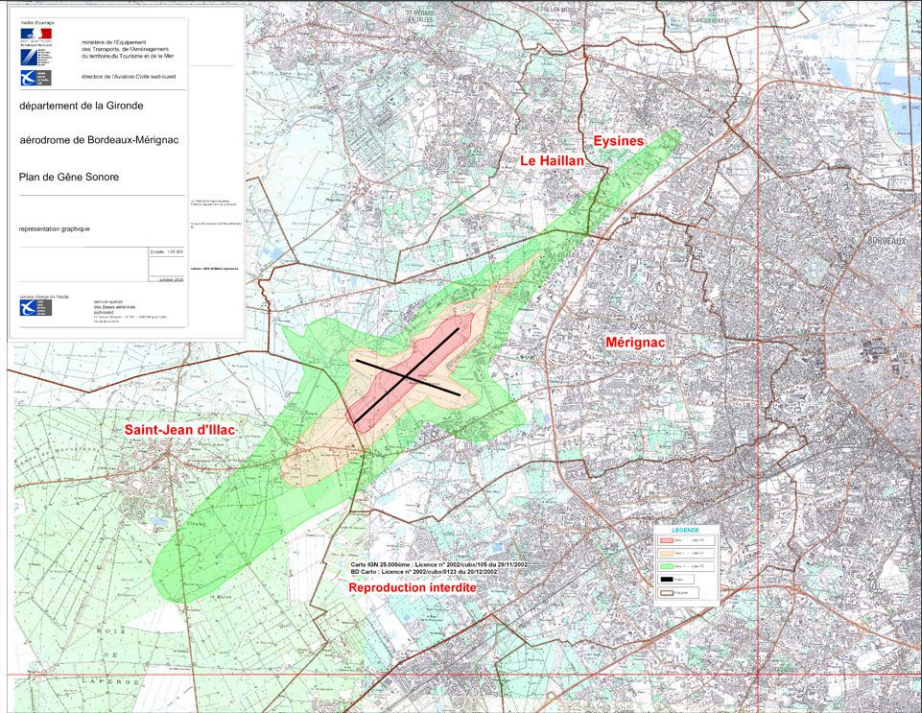
\includegraphics[width=.7\linewidth]{Images/pgs.png}  
    \caption{Plan de Gêne Sonore}
    \label{fig:pgs}
  \end{subfigure}
  \begin{subfigure}{0.45\textwidth}
    \centering
    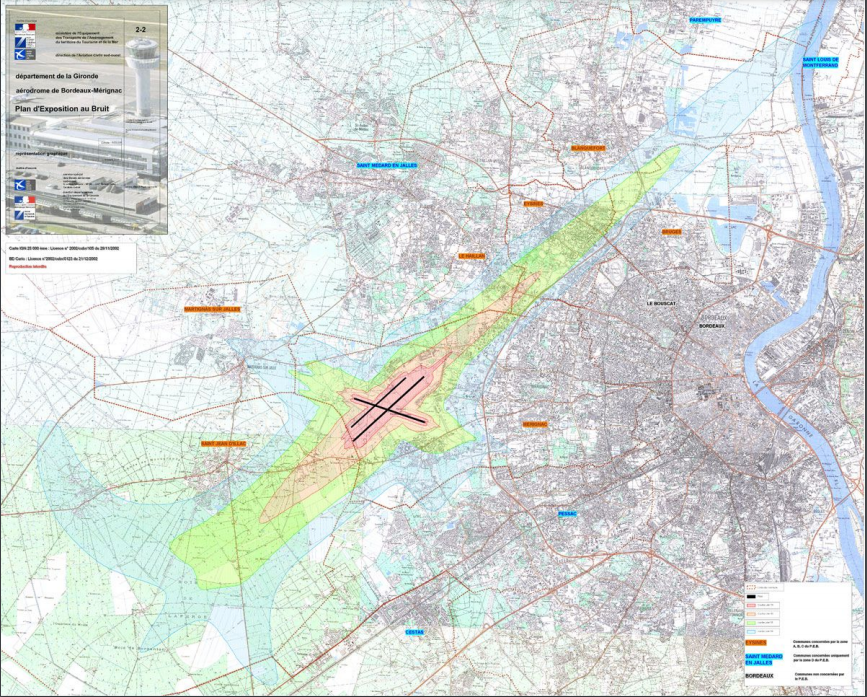
\includegraphics[width=.7\linewidth]{Images/peb}\newline
    \caption{Plan d'Exposition au Bruit}
    \label{fig:peb}
  \end{subfigure}
  \caption{Plans liés au bruit}
\label{fig:plans}
\end{figure}


Une autre action a été effectuée pour les riverains. La ville de Saint-Jean-D'Illac est située juste en dessous de la trajectoire de décollage de la piste la plus utilisée, les riverains se sont donc demandés si un changement de trajectoire pouvait être envisagé.
Le sujet a été étudié longuement et un problème majeur a été rencontré, si les aéronefs changeaient leurs trajectoires, ils devraient survoler une zone militaire, or c'est strictement interdit.
Une fois la trajectoire trouvée, il a fallu effectuer une demande aux services concernés, et au bout d'un an et demi cela a été accepté.\newline

Aujourd'hui, les avions remontant vers le nord effectuent leur virage bien plus au sud, et contournent donc la ville de Saint-Jean-D'Illac.\newline

%carte trajectoire

De plus, suite aux retours des riverains, l'Aéroport essaie de réduire les vols de nuit qui sont très gênants. Cependant ce n'est pas une tâche aisée puisque cela concerne également l'Aéroport de destination ou d'origine du vol.


\textbf{Environnement}

Le milieu aérien est un domaine très polluant et SA ADBM le sait. Un service est consacré à l'environnement, ils travaillent sur différents points comme les émissions carbones, la faune et flore environnante mais également d'autres sujets.


Des lois ont été mises en places au niveau des compagnies aériennes, par exemple, un passager peut s'il le souhaite choisir de compenser son émission carbone grâce à un don d'une valeur dépandant de la distance effectuée.
Une partie de cet argent est par la suite utilisé pour acheter des avions moins polluants ou reversé aux aéroports afin de réduire les émissions de la plateforme.\newline

SA ADBM prend ces enjeux très au sérieux, 8 millions d'euros ont été attribués pour réduire leur impact négatif sur l'environnement.
L'entreprise a également rejoint le programme Airport Carbon Accreditation (ACA). L'objectif de ce programme international est de rentre les plateformes aéroportuaires neutres en émissions carbones.
L'Aéroport de Bordeaux-Mérignac a validé le niveau 1 le 11 juin 2021, l'objectif de neutralité carbone est prévu pour 2030.

\begin{figure}[hbt!]
  \centering
  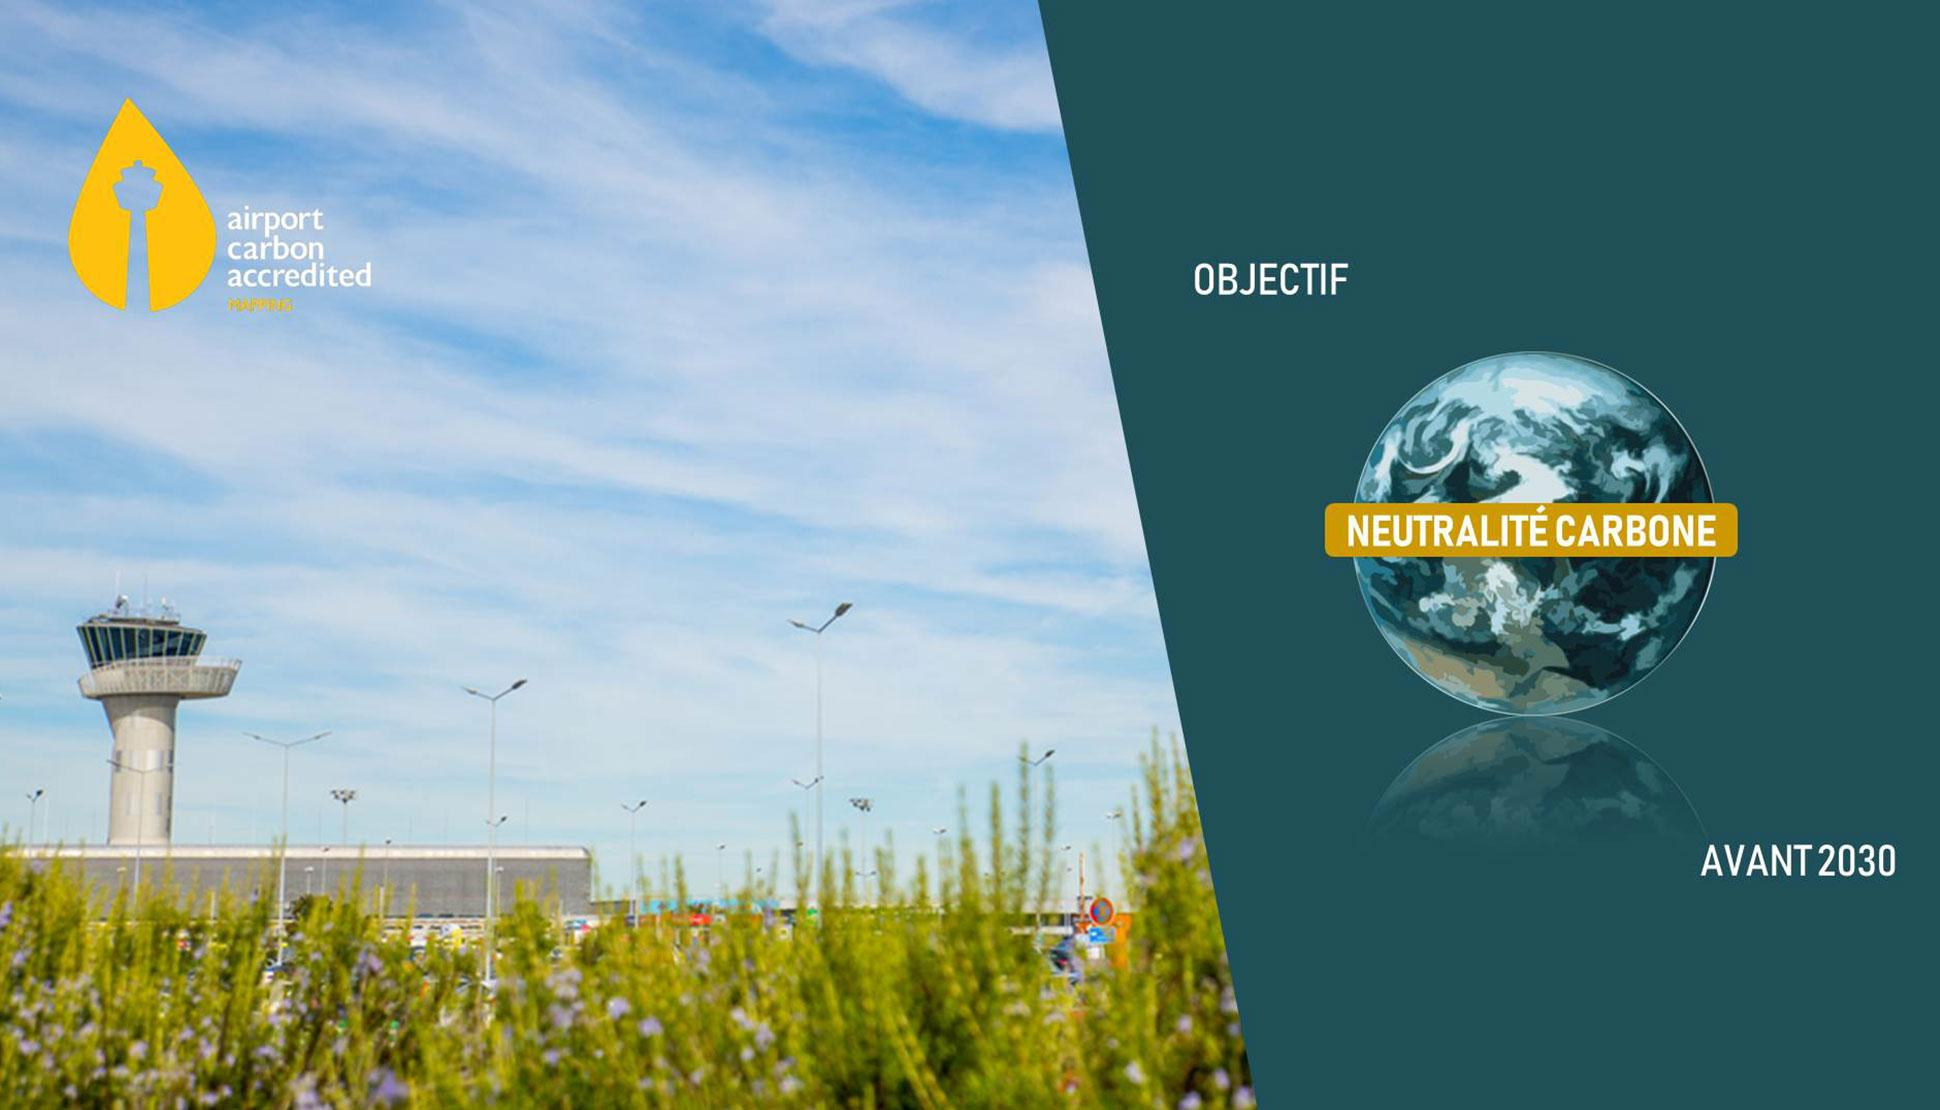
\includegraphics[width=12cm]{Images/aca2030.jpg}
  \caption{Airport Carbon Accreditation}
  \label{fig:aca2030}
\end{figure}


L'Aéroport ne s'arrête pas à ce seul programme, ils ont décidé d'agir de manière importante sur leurs activités afin de réduire leur pollution.

Concernant le côté ville, ils effectuent de petites actions comme le tri sélectif dans tout l'aéroport, pour le public mais également pour les salariés. SA ADBM rembourse 80\% du prix de l'abonnement de transports en communs aux salariés si celui-ci sert à venir travailler, afin de lutter contre la pollution des voitures.

SA ADBM possède de nombreux véhicules : Bus (navettes entre parkings), voitures de services, voitures d'astreintes. Tous ces véhicules polluent énormément et le service environnemental de l'aéroport le sait et une nouvelle règle a été instaurée : Lors d'un achat/remplacement de véhicule, celui-ci doit être électrique ou hybride (selon les besoins). Cela permettra de réduire leur consommation liée aux transports.\newline


Dans un objectif de réduction des émissions de carbone côté piste, la mise en place d’équipements d’alimentation en « 400 Hertz » a été effectuée en remplacement des groupes électrogènes de démarrage des avions stationnés au hall B et des passerelles du hall A.

De plus, tout nouveau bâtiment (comme le Satellite 3), doit être conduit avec la norme Haute Qualité Environnementale et selon des critères renforcés de qualité de service. Cela permettra de réduire leur consommation d'énergie sur le long terme.\newline


L'entreprise travaille également à la pose de panneaux photovoltaïques un peu partout sur la plateforme aéroportuaire : Façades des Halls A et B, Accès aux Parkings et près des pistes.

La plateforme aéroportuaire fait également attention à ses consommations d'eau. Des "Urinoirs Secs" ont été installés en 2019, et après 1 an ils ont permit d'économiser 1 million de litres d'eau, leur installation continue donc progressivement.
De plus, SA ADBM a un système de récupération d'eau de pluie et de récupération des eaux liées à l'entraînement des pompiers de la plateforme.\newline

La végétalisation est un projet qui est tenu à coeur par les responsables environnement. Lors de l'arrivée du Tramway en 2022, les abords seront végétalisés avec l'exigeance « zéro phytosanitaire »

La faune et la flore sont des points très importants lors de l'évolution des infrastructures. Avant de lancer une construction, SA ADBM fait intervenir un prestataire afin de réaliser une étude du terrain et étudier les conséquences sur l'environnement.
Concernant le projet "45ème Parallèle", c'est "Thallium" qui s'en est chargé. Ils étudient la faune et la flore locale et éditent un rapport sur ce qui doit être fait avant la construction.

Voici une carte réalisée pour ce projet :

\begin{figure}[hbt!]
  \centering
  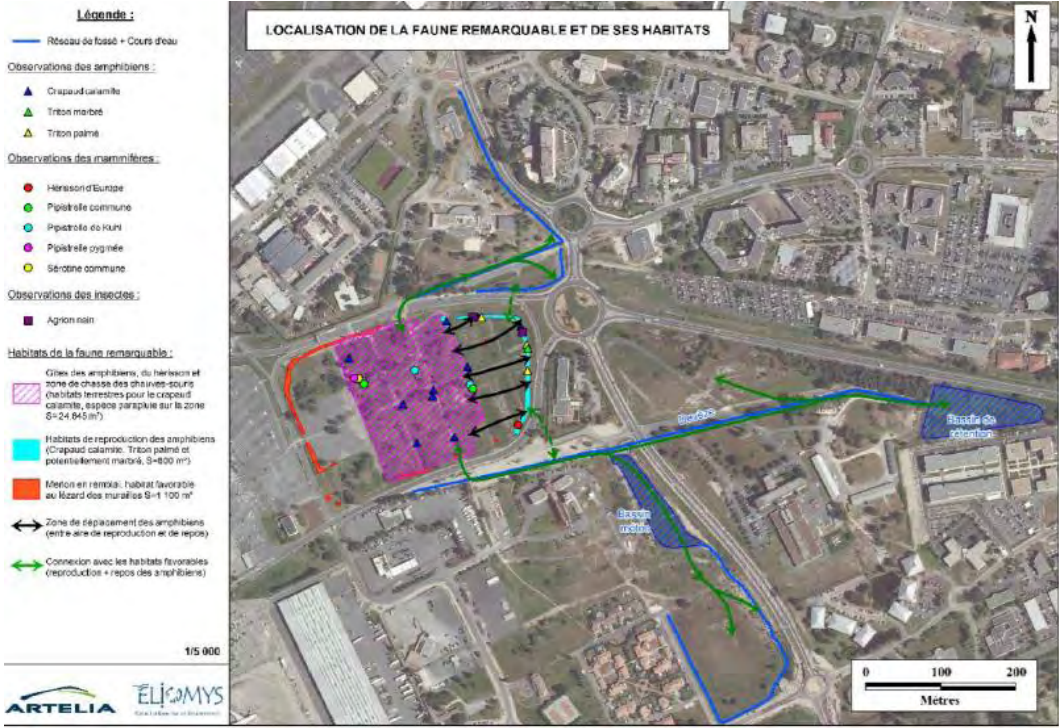
\includegraphics[width=14cm]{Images/carteenvironnement.png}
  \caption{Carte de localisation de la faune et de la flore}
  \label{fig:crapeau}
\end{figure}

Concernant la faune, SA ADBM a également installé des ruches dans un endroit végétalisé éloigné de la vue du public, une population de 150 000 abeilles s'y est installée et des ruches additionnelles ont été rajoutées. Des apiculteurs viennent régulièrement s'occuper des ruches, et d'ici quelques mois plusieurs kilogrammes de miel de l'Aéroport de Bordeaux-Mérignac existera.

 \begin{figure}[hbt!]
   \centering
   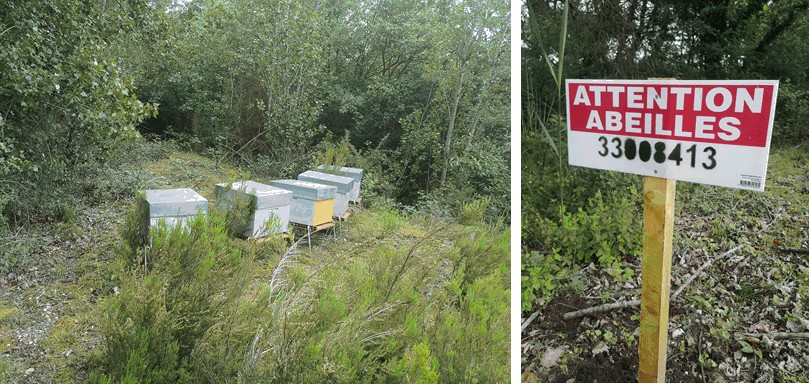
\includegraphics[width=14cm]{Images/ruches.jpg}
   \caption{Ruches}
   \label{fig:abeilles}
 \end{figure}

